\documentclass{article}
\usepackage{xeCJK}
 
\usepackage{iclr2022_conference,times}
\renewcommand*\ttdefault{cmtt}
\usepackage{hyperref}
\usepackage{url}
\usepackage{mathtools,amssymb}
\usepackage{pgfplots,pgfplotstable}
\pgfplotsset{compat=1.14}
\usepackage{array,colortbl}
\usepackage{xcolor}
\usepackage{algorithm,algorithmicx,algpseudocode}
\usepackage[capitalise]{cleveref}
\usepackage{caption}
\usepackage{graphbox}
\usepackage{placeins}
\usepackage{wrapfig}
\usepackage{subcaption}
\usepackage{etoolbox}
\usepackage{booktabs}       
\usepackage{microtype}      
\usepackage{adjustbox}
\usepackage[bottom]{footmisc}
\newcommand{\vardbtilde}[1]{\tilde{\raisebox{0pt}[0.85\height]{$\tilde{#1}$}}}
\newcommand{\defeq}{\coloneqq}
\newcommand{\grad}{\nabla}
\newcommand{\E}{\mathbb{E}}
\newcommand{\Var}{\mathrm{Var}}
\newcommand{\Cov}{\mathrm{Cov}}
\newcommand{\Ea}[1]{\E\left[#1\right]}
\newcommand{\Eb}[2]{\E_{#1}\!\left[#2\right]}
\newcommand{\Vara}[1]{\Var\left[#1\right]}
\newcommand{\Varb}[2]{\Var_{#1}\left[#2\right]}
\newcommand{\kl}[2]{D_{\mathrm{KL}}\!\left(#1 ~ \| ~ #2\right)}
\newcommand{\pdata}{{p_\mathrm{data}}}
\newcommand{\bA}{\mathbf{A}}
\newcommand{\bI}{\mathbf{I}}
\newcommand{\bJ}{\mathbf{J}}
\newcommand{\bH}{\mathbf{H}}
\newcommand{\bL}{\mathbf{L}}
\newcommand{\bM}{\mathbf{M}}
\newcommand{\bQ}{\mathbf{Q}}
\newcommand{\bR}{\mathbf{R}}
\newcommand{\bzero}{\mathbf{0}}
\newcommand{\bone}{\mathbf{1}}
\newcommand{\bb}{\mathbf{b}}
\newcommand{\bc}{\mathbf{c}}
\newcommand{\bd}{\mathbf{d}}
\newcommand{\be}{\mathbf{e}}
\newcommand{\bu}{\mathbf{u}}
\newcommand{\bv}{\mathbf{v}}
\newcommand{\bw}{\mathbf{w}}
\newcommand{\bx}{\mathbf{x}}
\newcommand{\by}{\mathbf{y}}
\newcommand{\bz}{\mathbf{z}}
\newcommand{\bxh}{\hat{\mathbf{x}}}
\newcommand{\btheta}{{\boldsymbol{\theta}}}
\newcommand{\bphi}{{\boldsymbol{\phi}}}
\newcommand{\bepsilon}{{\boldsymbol{\epsilon}}}
\newcommand{\bmu}{{\boldsymbol{\mu}}}
\newcommand{\bnu}{{\boldsymbol{\nu}}}
\newcommand{\bSigma}{{\boldsymbol{\Sigma}}}
\newtheorem{lemma}{Lemma}
\newtheorem{theorem}{Theorem}
\DeclareMathOperator{\snr}{SNR}
\DeclareMathOperator{\sigmoid}{sigmoid}
\DeclareMathOperator{\expm1}{expm1}
\DeclareMathOperator{\softplus}{softplus}
\title{
无分类器扩散制导}
\author{Jonathan Ho  \&  Tim Salimans  \\ 
Google Research, Brain team \\ 
\texttt{ \{ jonathanho,salimans \} @google.com}
}
\newcommand{\fix}{\marginpar{FIX}}
\newcommand{\new}{\marginpar{NEW}}
\iclrfinalcopy 
\begin{document}




 \maketitle 


 \begin{abstract}
分类器指导是最近引入的一种方法,用于权衡条件扩散模型训练后的模式覆盖率和样本保真度,与其他类型生成模型中的低温采样或截断相同。分类器指导将扩散模型的分数估计与图像分类器的梯度相结合,从而需要训练与扩散模型分开的图像分类器。它还提出了一个问题,即是否可以在没有分类器的情况下进行指导。我们证明了在没有这样的分类器的情况下,指导确实可以通过纯生成模型来执行:在我们所说的无分类器指导中,我们联合训练条件和无条件扩散模型,并将得到的条件和无条件分数估计结合起来,以获得样本质量和多样性之间的权衡,类似于使用分类器指导所获得的结果。 \let   \thefootnote   \relax   \footnote{
本文的一个简短版本出现在关于深层生成模型和下游应用的NeurIPS2021年研讨会上: \url{https://openreview.net/pdf?id=qw8AKxfYbI} } 
\end{abstract} 


 \section{
引言} 
 \label{sec:introduction} 


 \setlength{\tabcolsep}   {0.5pt} 
 \begin{figure}[b]\centering
\begin{tabular}{lccr}
\adjincludegraphics[width=0.86\textwidth,Clip={0.5\width} {0.427\height} {0.212\width} {0\height}]{images/guidance_figure_1_minus0.jpg} &
\adjincludegraphics[width=0.86\textwidth,Clip={0.5\width} {0.427\height} {0.212\width} {0\height}]{images/guidance_figure_2_minus1.jpg} &
\adjincludegraphics[width=0.86\textwidth,Clip={0.5\width} {0.427\height} {0.212\width} {0\height}]{images/guidance_figure_3_minus2.jpg} &
\adjincludegraphics[width=0.86\textwidth,Clip={0.5\width} {0.427\height} {0.212\width} {0\height}]{images/guidance_figure_4_minus3.jpg}
\end{tabular}
\caption{
64x64 ImageNet扩散模型的无分类器指导。从左到右:从左侧的非引导样本开始,增加无分类器的指导量。}
\label{fig:dog_guidance}
\end{figure} 
 \setlength{\tabcolsep}   {6pt} 


 \begin{figure}[t] \centering

\includegraphics[width=\linewidth]{images/guided_gaussian_mixture.png}
\caption{
指导对三个高斯混合的影响,每个混合分量代表以一个类别为条件的数据。最左边的地块是非引导边际密度。从左到右是随引导强度增加的归一化引导条件的混合密度。}
\label{fig:gaussian_guidance}
\end{figure} 


扩散模型是最近出现的一类富有表现力和灵活性的生成模型,在图像和音频合成任务中提供具有竞争力的样本质量和似然分数~ \citep{sohl2015deep,song2019generative,ho2020denoising,song2020score,kingma2021variational,song2021maximum} 。这些模型以相当少的推理步骤~ \citep{chen2020wavegrad,kong2020diffwave} 提供了与自回归模型质量相媲美的音频合成性能,并且它们提供的图像网生成结果在FID分数和分类准确率分数~ \citep{ho2021cascaded,dhariwal2021diffusion} 方面优于BigGan-Deep~ \citep{brock2018large} 和VQ-VAe-2~ \citep{razavi2019generating} 。


 \citet{dhariwal2021diffusion} 提出了 \emph{classifier guidance} ,这是一种使用额外训练的分类器来提高扩散模型的样本质量的技术。在分类器指导之前,人们不知道如何从类似于截断的BigGan~ \citep{brock2018large} 或低温Glow~ \citep{kingma2018glow} 产生的扩散模型中产生“低温”样本。幼稚的尝试,例如缩放模型分数向量或减少扩散采样期间添加的高斯噪声量,是无效的~ \citep{dhariwal2021diffusion} 。相反,分类器指导将扩散模型的分数估计与分类器的对数概率的输入梯度混合在一起。通过改变分类器梯度的强度, \citeauthor{dhariwal2021diffusion} 可以在初始分数~ \citep{salimans2016improved} 和FID分数~ \citep{heusel2017gans} (或准确率和召回率)之间进行权衡,其方式类似于改变BigGAN的截断参数。


我们感兴趣的是,是否可以在没有分类器的情况下执行分类器指导。分类器指导使扩散模型训练流水线复杂化,因为它需要训练额外的分类器,并且该分类器必须在有噪声的数据上训练,因此通常不可能插入预先训练的分类器。此外,由于分类器引导在采样期间混合了分数估计和分类器梯度,因此分类器引导的扩散采样可以被解释为试图将图像分类器与基于梯度的对抗性攻击相混淆。这提出了一个问题,即分类器指导是否成功地提升了基于分类器的指标,例如FID和初始得分(IS),因为它与这些分类器是对抗性的。在分类器梯度方向上的步进也与GAN训练有一些相似之处,特别是对于非参数生成器;这也提出了一个问题,即分类器引导的扩散模型在基于分类器的指标上是否表现良好,因为它们开始类似于已知在此类指标上表现良好的GAN。


为了解决这些问题,我们提出了一种完全避免任何分类器的制导方法 \emph{classifier-free guidance} 。无分类器指导不是沿着图像分类器的梯度方向采样,而是将条件扩散模型和联合训练的无条件扩散模型的分数估计混合在一起。通过扫过混合权重,我们获得了类似于分类器指导所获得的FID/IS折衷。我们的无分类器指导结果表明,与其他类型的生成模型一样,纯生成扩散模型能够合成极高保真度的样本。


 \section{
背景} 
 \label{sec:background} 我们在连续时间训练扩散模型~ $\bz =  \{ \bz_\lambda \,|\, \lambda \in [\lambda_{\mathrm{min}}, \lambda_{\mathrm{max}}] \} $ :设 $\bx \sim p(\bx)$ 和 $\bz =  \{ \bz_\lambda \,|\, \lambda \in [\lambda_{\mathrm{min}}, \lambda_{\mathrm{max}}] \} $ 为超参数 $\lambda_{\mathrm{min}} < \lambda_{\mathrm{max}} \in \mathbb{R}$ ,正向过程 $q(\bz|\bx)$ 是保方差马尔可夫过程~ \citep{sohl2015deep} :
 \begin{align}
q(\bz_\lambda|\bx) &= \mathcal{N}(\alpha_\lambda \bx, \sigma_\lambda^2 \bI),  \  \text{where} \  \alpha_\lambda^2 = 1/(1+e^{-\lambda}), \  \sigma_\lambda^2 = 1-\alpha_\lambda^2  \\ 
q(\bz_{\lambda} | \bz_{\lambda'}) &= \mathcal{N}((\alpha_{\lambda}/\alpha_{\lambda'})\bz_{\lambda'}, \sigma_{\lambda|\lambda'}^2\bI),  \  \text{where} \  \lambda < \lambda', \  
\sigma^2_{\lambda|\lambda'} = (1-e^{\lambda-\lambda'})\sigma_\lambda^2 
\end{align} 我们将使用符号 $p(\bz)$ (或 $p(\bz_\lambda)$ )来表示当 $\bx \sim p(\bx)$ 和 $\bz \sim q(\bz|\bx)$ 时 $\bz$ (或 $\bz_\lambda$ )的边缘。请注意, $\lambda = \log \alpha_\lambda^2/\sigma_\lambda^2$ ,因此 $\lambda$ 可以解释为 $\bz_\lambda$ 的对数信噪比,并且正向过程沿 $\lambda$ 递减的方向运行。


在 $\bx$ 的条件下,正向过程可以用跃迁来描述
 $q(\bz_{\lambda'}|\bz_\lambda,\bx) = \mathcal{N}(\tilde\bmu_{\lambda'|\lambda}(\bz_\lambda,\bx), \tilde\sigma^2_{\lambda'|\lambda}\bI)$ ,其中
 \begin{align}
\tilde\bmu_{\lambda'|\lambda}(\bz_\lambda,\bx) = e^{\lambda-\lambda'}(\alpha_{\lambda'}/\alpha_{\lambda})\bz_\lambda + (1-e^{\lambda - \lambda'})\alpha_{\lambda'}\bx,
\quad \tilde\sigma^2_{\lambda'|\lambda} = (1-e^{\lambda-\lambda'})\sigma_{\lambda'}^2
\end{align} 逆过程生成模型从 $p_\theta(\bz_{\lambda_{\mathrm{min}}}) = \mathcal{N}(\bzero, \bI)$ 开始。我们指定转换:
 \begin{align}p_\theta(\bz_{\lambda'}|\bz_{\lambda}) = \mathcal{N}(\tilde\bmu_{\lambda'|\lambda}(\bz_\lambda,\bx_\theta(\bz_\lambda)),  (\tilde\sigma^2_{\lambda'|\lambda})^{1-v} (\sigma^2_{\lambda|\lambda'})^v)\end{align} 在采样过程中,我们沿着递增序列 $\lambda_{\mathrm{min}} = \lambda_1 < \cdots < \lambda_T = \lambda_{\mathrm{max}}$ 对 $T$ 时间步长应用这种转变;换句话说,我们遵循离散时间祖先采样器~???。如果模型 $\bx_\theta$ 是正确的,则作为 $T\rightarrow\infty$ ,我们从样本路径分布为 $p(\bz)$ ~ \citep{song2020score} 的随机过程中获得样本,并用 $p_\theta(\bz)$ 来表示连续时间模型分布。方差是 $\tilde\sigma^2_{\lambda'|\lambda}$ 和 $\sigma^2_{\lambda|\lambda'}$ 的对数空间内插,由~ \citet{nichol2021improved} 提出;我们发现使用常量超参数 $v$ 比使用学习的 $\bz_\lambda$ 依赖的 $v$ 更有效。请注意,方差简化为 $\tilde\sigma^2_{\lambda'|\lambda}$ 作为 $\lambda'\rightarrow\lambda$ ,因此 $v$ 仅在实际使用非无穷小时间步长进行采样时才有效。


反向过程平均值来自估计 $\bx_\theta(\bz_\lambda) \approx \bx$ 插入到 $q(\bz_{\lambda'}|\bz_\lambda,\bx)$ ~ \citep{ho2020denoising,kingma2021variational} 中( $\bx_\theta$ 也接受 $\lambda$ 作为输入,但为了保持符号的整洁,我们取消了这一输入)。我们将 $\bx_\theta$ 参数化为 $\bepsilon$ -预测~ \citep{ho2020denoising} : $\bx_\theta(\bz_\lambda) = (\bz_\lambda - \sigma_\lambda \bepsilon_\theta(\bz_\lambda)) / \alpha_\lambda$ ,并针对目标进行训练
 \begin{align}
    \Eb{\bepsilon,\lambda}{\|\bepsilon_\theta(\bz_\lambda) - \bepsilon \|^2_2}
\end{align} ,其中 $\bepsilon\sim\mathcal{N}(\bzero,\bI)$ 、 $\bz_\lambda = \alpha_\lambda\bx + \sigma_\lambda\bepsilon$ 和 $\lambda$ 取自 $[\lambda_{\mathrm{min}}, \lambda_{\mathrm{max}}]$ 上的分布 $p(\lambda)$ 。这个目标是在多个噪声尺度~ \citep{song2019generative} 上去噪匹配~ \citep{vincent2011connection,hyvarinen2005estimation} 的分数,当 $p(\lambda)$ 是均匀的时,目标与潜变量模型 $\int p_\theta(\bx|\bz) p_\theta(\bz) d\bz$ 的边际对数似然的变分下界成比例,忽略未指定解码器 $p_\theta(\bx|\bz)$ 的项和 $\bz_{\lambda_\mathrm{min}}$ ~ \citep{kingma2021variational} 处的先验项。


如果 $p(\lambda)$ 不一致,则目标可以解释为加权变分下界,其权重可以根据样本质量~ \citep{ho2020denoising,kingma2021variational} 进行调整。我们使用的 $p(\lambda)$ 来自于 \citet{nichol2021improved} 的离散时间余弦噪声调度:对于均匀分布的 $u \in [0,1]$ ,我们通过 $\lambda = -2\log\tan(au+b)$ 采样 $\lambda$ ,其中 $b = \arctan(e^{-\lambda_{\mathrm{max}}/2})$ 和 $a = \arctan(e^{-\lambda_{\mathrm{min}}/2}) - b$ 。这表示修改为在有界区间上支持的双曲正割分布。对于有限时间步生成,我们使用 $\lambda$ 值对应于均匀间隔的 $u \in [0, 1]$ ,最终生成的样本是 $\bx_\theta(\bz_{\lambda_\mathrm{max}})$ 。


由于 $\bepsilon_\theta(\bz_\lambda)$ 的损失是对所有 $\lambda$ 的分数匹配进行去噪,所以我们的模型学习的分数 $\bepsilon_\theta(\bz_\lambda)$ 估计了噪声数据 $\bz_\lambda$ 的分布的对数密度的梯度,即 $\bepsilon_\theta(\bz_\lambda) \approx -\sigma_\lambda \nabla_{\bz_\lambda}\log p(\bz_\lambda)$ ;然而,请注意,因为我们使用无约束神经网络来定义 $\bepsilon_\theta$ ,所以不需要存在任何梯度为 $\bepsilon_\theta$ 的标量势。从学习的扩散模型中采样类似于使用朗之万式扩散从收敛于原始数据 $\bx$ 的条件分布 $p(\bx)$ 的分布序列 $p(\bz_\lambda)$ 中采样。


在条件生成建模的情况下,数据 $\bx$ 与条件信息~ $\bc$ 、即用于类条件图像生成的类标签一起绘制。对该模型的唯一修改是反向过程函数近似器接收 $\bc$ 作为输入,与 $\bepsilon_\theta(\bz_\lambda, \bc)$ 中的一样。


 \section{
导向} 
 \label{sec:guidance} 


某些产生式模型的一个有趣的特性,例如GANS和基于流的模型,是通过减少在采样时间输入到产生式模型的噪声的方差或范围来执行截断或低温采样的能力。其预期效果是减少样本的多样性,同时提高每个样本的质量。例如,BigGAN~ \citep{brock2018large} 中的截断分别在低截断量和高截断量下产生了FID值和初始值之间的权衡曲线。GLOW~ \citep{kingma2018glow} 中的低温采样也有类似的效果。


不幸的是,在扩散模型中实施截断或低温抽样的直接尝试是无效的。例如,在反向过程中缩放模型分数或减小高斯噪声的方差会导致扩散模型生成模糊、低质量的样本~ \citep{dhariwal2021diffusion} 。


 \subsection{
分类器制导} 


为了在扩散模型中获得类似截断的效果, \citet{dhariwal2021diffusion} 引入了 \emph{classifier guidance} ,其中,将扩散分数 $\bepsilon_\theta(\bz_\lambda, \bc) \approx -\sigma_\lambda \nabla_{\bz_\lambda}\log p(\bz_\lambda |  \bc)$ 修改为包括辅助分类器模型 $p_{\theta}(\bc | \bz_\lambda)$ 的对数似然梯度,如下所示:
 \[
\tilde{\bepsilon}_\theta(\bz_\lambda, \bc) = \bepsilon_\theta(\bz_\lambda, \bc) - w\sigma_{\lambda}\nabla_{\bz_\lambda}\log p_{\theta}(\bc | \bz_\lambda) \approx -\sigma_{\lambda}\nabla_{\bz_\lambda}[\log p(\bz_\lambda |  \bc) + w \log p_{\theta}(\bc | \bz_\lambda) ],
\] ,其中 $w$ 是控制分类器指导的强度的参数。然后,当从扩散模型中采样时,使用该修改的分数 $\tilde{\bepsilon}_\theta(\bz_\lambda, \bc)$ 来代替 $\bepsilon_\theta(\bz_\lambda, \bc)$ ,从而得到来自分布的近似样本
 \[\tilde{p}_{\theta}(\bz_\lambda | \bc) \propto p_{\theta}(\bz_\lambda | \bc)p_{\theta}(\bc | \bz_\lambda)^{w}.\] 其效果是对分类器 $p_{\theta}(\bc | \bz_\lambda)$ 为其赋予正确标签的高似然性的数据的概率进行向上加权:可以很好地分类的数据在感知质量的初始分数 \citep{salimans2016improved} 上得分很高,这是通过设计来奖励生成模型的。因此, \citeauthor{dhariwal2021diffusion} 发现,通过设置 $w > 0$ ,他们可以提高其扩散模型的初始分数,但代价是其样本的多样性降低。


 \Cref{fig:gaussian_guidance} 说明了数值求解导引 $\tilde{p}_{\theta}(\bz_\lambda | \bc) \propto p_{\theta}(\bz_\lambda | \bc)p_{\theta}(\bc | \bz_\lambda)^{w}$ 对三个类的玩具2D算例的影响,其中每个类的条件分布是各向同性的高斯分布。应用指导的每个条件的形式都是明显的非高斯的。随着引导强度的增加,每个条件质量都将概率质量放置在远离其他类别的位置,并朝着Logistic回归给出的高置信度方向移动,并且大多数质量变得集中在较小的区域。这种行为可以被看作是在ImageNet模型中增加分类器指导强度时发生的初始分数增加和样本多样性减少的简化表现。


将具有权重 $w+1$ 的分类器指导应用于无条件模型理论上将导致与将具有权重 $w$ 的分类器指导应用于条件模型相同的结果,因为 $p_{\theta}(\bz_\lambda | \bc)p_{\theta}(\bc | \bz_\lambda)^{w} \propto p_{\theta}(\bz_\lambda)p_{\theta}(\bc | \bz_\lambda)^{w+1}$ ;或者根据分数,
 \begin{align*}
\bepsilon_\theta(\bz_\lambda) - (w+1)\sigma_{\lambda}\nabla_{\bz_\lambda}\log p_{\theta}(\bc | \bz_\lambda) &\approx -\sigma_{\lambda}\nabla_{\bz_\lambda}[\log p(\bz_\lambda) + (w+1) \log p_{\theta}(\bc | \bz_\lambda) ]  \\ 
&= -\sigma_{\lambda}\nabla_{\bz_\lambda}[\log p(\bz_\lambda|\bc) + w\log p_{\theta}(\bc | \bz_\lambda) ],
\end{align*} ,但有趣的是, \citeauthor{dhariwal2021diffusion} 在将分类器指导应用于已经有类的条件模型时获得了最佳结果,而不是将指导应用于无条件模型。出于这个原因,我们将继续指导一个已经有条件的模型的设置。


 \subsection{
无分类器制导} 


虽然分类器引导在截断或低温采样中成功地权衡了IS和FID,但它仍然依赖于图像分类器的梯度,我们出于~ \cref{sec:introduction} 中所述的原因寻求消除该分类器。这里,我们描述了 \emph{classifier-free guidance} ,它在没有这种梯度的情况下达到了同样的效果。无分类器指导是修改 $\bepsilon_\theta(\bz_\lambda, \bc)$ 的另一种方法,使其具有与分类器指导相同的效果,但没有分类器。 \cref{alg:training,alg:sampling} 详细描述了无分类器指导下的训练和采样。


 \begin{algorithm}[tb]
  \caption{
联合训练无分类器引导的扩散模型} \label{alg:training}
  \begin{algorithmic}[1]
    \Require     $p_\mathrm{uncond}$    : probability of unconditional training
    \Repeat
      \State     $(\bx,\bc) \sim p(\bx,\bc)$     \Comment{Sample data with conditioning from the dataset}
      \State     $\bc \gets \varnothing$     with probability     $p_\mathrm{uncond}$     \Comment{Randomly discard conditioning to train unconditionally}
      \State     $\lambda \sim p(\lambda)$     \Comment{Sample log SNR value}
      \State     $\bepsilon\sim\mathcal{N}(\bzero,\bI)$    
      \State     $\bz_\lambda = \alpha_\lambda\bx + \sigma_\lambda \bepsilon$     \Comment{Corrupt data to the sampled log SNR value}
      \State Take gradient step on     $\grad_\theta \left\| \bepsilon_\theta(\bz_\lambda,\bc) - \bepsilon \right\|^2$     \Comment{Optimization of denoising model}
    \Until{converged}
  \end{algorithmic}
\end{algorithm} 


 \begin{algorithm}[tb]
  \caption{
无分类器引导的条件采样} \label{alg:sampling}
  \begin{algorithmic}[1]
    \Require     $w$    : guidance strength
    \Require     $\bc$    : conditioning information for conditional sampling
    \Require     $\lambda_1, \dotsc, \lambda_T$    : increasing log SNR sequence with      $\lambda_1=\lambda_{\mathrm{min}}$    ,      $\lambda_T=\lambda_{\mathrm{max}}$    
    \State     $\bz_{1} \sim \mathcal{N}(\bzero, \bI)$    
    \For{    $t=1, \dotsc, T$    }

          $\!\!\triangleright$     Form the classifier-free guided score at log SNR     $\lambda_t$    
      \State     $\tilde{\bepsilon}_t = (1+w)\bepsilon_\theta(\bz_{t}, \bc) - w\bepsilon_{\theta}(\bz_{t})$     

          $\!\!\triangleright$     Sampling step (could be replaced by another sampler, e.g. DDIM)
      \State     $\tilde\bx_t = (\bz_{t}-\sigma_{\lambda_t}\tilde\bepsilon_t)/\alpha_{\lambda_t}$    
      \State     $\bz_{t+1} \sim \mathcal{N}(\tilde\bmu_{\lambda_{t+1}|\lambda_t}(\bz_{t},\tilde\bx_t),  (\tilde\sigma^2_{\lambda_{t+1}|\lambda_t})^{1-v} (\sigma^2_{\lambda_t|\lambda_{t+1}})^v)$     if     $t<T$     else     $\bz_{t+1}=\tilde\bx_t$    
    \EndFor
    \State \textbf{return}     $\bz_{T+1}$    
  \end{algorithmic}
\end{algorithm} 


我们没有训练单独的分类器模型,而是选择训练无条件去噪扩散模型 $p_{\theta}(\bz)$ 和条件模型 $p_{\theta}(\bz | \bc)$ ,其中无条件去噪扩散模型 $p_{\theta}(\bz)$ 通过得分估计器 $\bepsilon_{\theta}(\bz_\lambda)$ 参数化,条件模型 $p_{\theta}(\bz | \bc)$ 通过 $\bepsilon_{\theta}(\bz_\lambda, \bc)$ 参数化。我们使用单个神经网络来参数化这两个模型,其中对于无条件模型,我们只需在预测分数时为类标识符 $\bc$ 输入空令牌 $\varnothing$ ,即XMATHX SP  $\bepsilon_{\theta}(\bz_\lambda) = \bepsilon_{\theta}(\bz_\lambda, \bc = \varnothing)$ 。我们简单地通过将 $\bc$ 随机设置为无条件类标识符 $\varnothing$ 以一定概率 $p_\mathrm{uncond}$ 设置为超参数来简单地联合训练无条件模型和条件模型。(当然可以单独训练模型,而不是联合训练它们在一起,但我们选择联合训练,因为它实施起来非常简单,不会使训练管道复杂化,也不会增加参数总数。)然后,我们使用以下有条件和无条件得分估计的线性组合来执行抽样:
 \begin{align}
    \tilde{\bepsilon}_\theta(\bz_\lambda, \bc) = (1+w)\bepsilon_\theta(\bz_\lambda, \bc) - w\bepsilon_{\theta}(\bz_\lambda) \label{eq:classifier_free_score}
\end{align} 
 \cref{eq:classifier_free_score} 不存在分类器梯度,因此在 $\tilde\bepsilon_\theta$ 方向上迈出一步不能解释为对图像分类器的基于梯度的对抗性攻击。此外,由于使用了无约束神经网络, $\tilde\bepsilon_\theta$ 是由非保守向量场的分数估计构造的,因此通常不存在以 $\tilde\bepsilon_\theta$ 为分类器引导分数的标量势,例如分类器对数似然。


尽管通常可能不存在以 \cref{eq:classifier_free_score} 为分类器指导分数的分类器,但它实际上是由隐式分类器 $p^{i}(\bc | \bz_\lambda) \propto p(\bz_\lambda | \bc)/p(\bz_\lambda)$ 的梯度启发的。如果我们可以获得确切的分数 $\bepsilon^*(\bz_\lambda, \bc)$ 和 $\bepsilon^*(\bz_\lambda)$ (分别属于 $p(\bz_\lambda|\bc)$ 和 $p(\bz_\lambda)$ ),则该隐式分类器的梯度将是 $\nabla_{\bz_\lambda} \log p^{i}(\bc | \bz_\lambda) = -\frac{1}{\sigma_{\lambda}}[\bepsilon^*(\bz_\lambda, \bc) - \bepsilon^*(\bz_\lambda)]$ ,并且使用该隐式分类器的分类器指导将把分数估计修改为 $\tilde{\bepsilon}^*(\bz_\lambda, \bc) = (1+w)\bepsilon^*(\bz_\lambda, \bc) - w\bepsilon^*(\bz_\lambda)$ 。请注意与 \cref{eq:classifier_free_score} 的相似之处,但也要注意 $\tilde{\bepsilon}^*(\bz_\lambda,\bc)$ 与 $\tilde{\bepsilon}_\theta(\bz_\lambda,\bc)$ 的根本不同。前者是由尺度分类器梯度 $\bepsilon^*(\bz_\lambda, \bc) - \bepsilon^*(\bz_\lambda)$ 构造的,后者是由估计 $\bepsilon_\theta(\bz_\lambda, \bc) - \bepsilon_\theta(\bz_\lambda)$ 构造的,并且该表达式一般不是任何分类器的(尺度)梯度,同样,因为得分估计是无约束神经网络的输出。


使用贝叶斯规则对生成模型进行倒置会产生一个提供有用指导信号的好的分类器,这并不是一个明显的先验。例如, \cite{grandvalet2004semi} 发现,即使在生成模型的规格与数据分布完全匹配的人工情况下,判别模型的性能通常也优于从生成模型派生的隐式分类器。在像我们这样的情况下,我们预计模型会被错误指定,根据贝叶斯规则导出的分类器可能不一致~ \citep{grunwald2007suboptimal} ,并且我们失去了对它们性能的所有保证。然而,在 \cref{sec:experiments} 中,我们的经验表明,无分类器引导能够折衷FID,并且与分类器引导相同。在 \cref{sec:discussion} 中,我们讨论了无量词制导相对于量词制导的含义。


 \section{
实验} 
 \label{sec:experiments} 


 \begin{figure}[tb] \centering
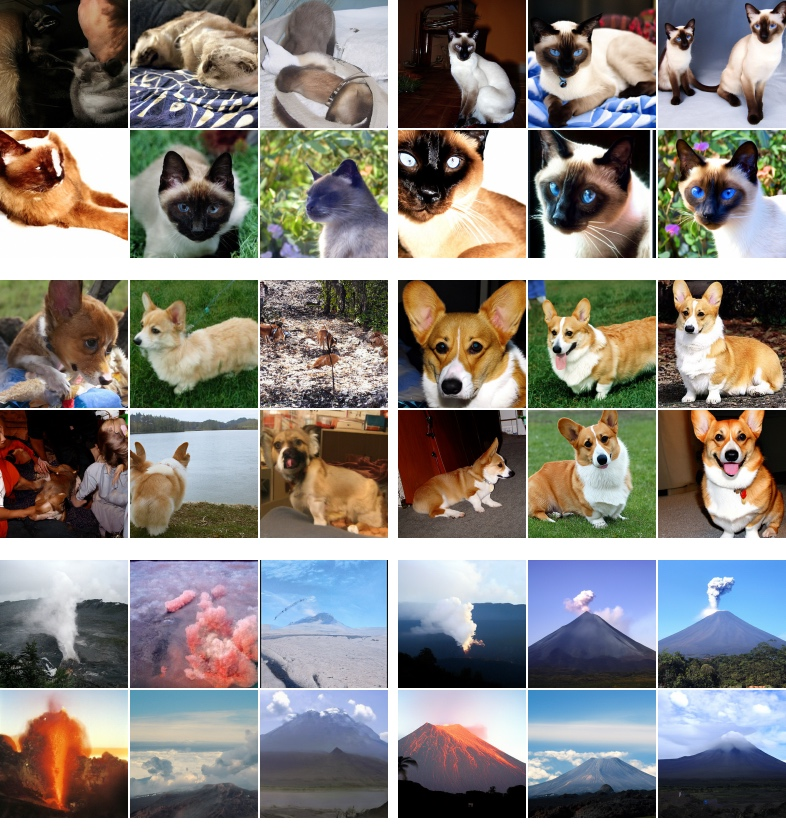
\includegraphics[width=\linewidth]{images/i128_guidance_2.jpg}
\vspace{-2em}
\caption{
128x128 ImageNet上的无分类器指南。左:非引导样本,右:具有 $w=3.0$ 的无分类器引导样本。有趣的是,像这样的强引导样本显示出饱和的颜色。有关更多信息,请参阅 \cref{fig:i128_guidance_more} 。}
\label{fig:i128_guidance}
\end{figure} 


我们从BigGAN论文~ \citep{brock2018large} 开始,在面积下采样的类条件图像网~ \citep{russakovsky2015imagenet} 上训练扩散模型,该模型是研究FID和初始分数之间权衡的标准设置。


我们实验的目的是作为概念的证明,以证明无分类器指导能够达到类似于分类器指导的FID/IS折衷,并理解无分类器指导的行为,而不一定在这些基准上推动样本质量度量达到最先进的水平。为此,我们使用与 \citet{dhariwal2021diffusion} 的引导扩散模型相同的模型体系结构和超参数(除了 \cref{sec:background} 中规定的连续时间训练);这些超参数设置针对分类器指导进行了调整,因此对于无分类器指导可能是次优的。此外,由于我们将条件模型和无条件模型摊销到相同的架构中,而不需要额外的分类器,因此实际上我们使用的模型容量比以前的工作更少。尽管如此,我们的无分类器指导模型仍然可以产生具有竞争力的样本质量指标,有时还会优于以前的工作,如以下各节所示。


 \subsection{
改变无分类器制导强度} 在实验上验证了本文的主要结论:无分类器制导能够以类似于分类器制导或GaN截断的方式折衷IS和FID。我们将我们提出的无分类器指导应用于 $64\times64$ 和 $128\times128$ 类条件图像网的生成。在 \cref{table:i64} 和 \cref{fig:i64_fid_is_plot} 中,我们在我们的 $64\times64$ ImageNet模型上展示了横扫制导强度 $w$ 的样本质量效应; \cref{table:i128} 和 \cref{fig:i128_fid_is_plot} 对于我们的 $128\times128$ 模型显示了相同的质量效应。我们考虑 $w \in  \{ 0, 0.1, 0.2, \ldots, 4 \} $ ,并按照 \citet{heusel2017gans} 和 \citet{salimans2016improved} 的步骤,对每个值使用50000个样本来计算FID和初始得分。所有型号均使用对数信噪比端点 $\lambda_\mathrm{min}=-20$ 和 $\lambda_\mathrm{max}=20$ 。 $64\times64$ 模型使用采样器噪声内插系数 $v=0.3$ ,训练了40万步; $128\times128$ 模型使用 $v=0.2$ ,训练了270万步。


根据数据集的不同,在少量引导( $w = 0.1$ 或 $w=0.3$ )的情况下获得最好的识别结果,而在强引导( $w \geq 4$ )的情况下获得最佳结果。在这两个极端之间,我们看到了这两个感知质量指标之间的明显权衡,FID单调减少,而 $w$ 单调增加。我们的结果与 \citet{dhariwal2021diffusion} 和 \citet{ho2021cascaded} 相比是有利的,事实上,我们的 $128\times128$ 结果是文献中最先进的。在 $w=0.3$ 时,我们的模型在 $128\times128$ ImageNet上的FID得分优于分类器引导的ADM-G;在 $w=4.0$ 时,我们的模型在FID和IS上都优于BigGan-Deep,当BigGan-Deep被评估为其最佳IS截断水平时。


 \Cref{fig:dog_guidance,fig:i64_samples,fig:i128_guidance,fig:i128_samples,fig:i128_guidance_more} 显示了我们的模型在不同的制导水平下随机生成的样本:在这里,我们清楚地看到,增加无分类器的制导强度具有减少样本种类和提高个体样本保真度的预期效果。


 \begin{table}[!htb]
\centering\small
\begin{tabular}{c|c|c}
\toprule
Model & FID (    $\downarrow$    ) & IS (    $\uparrow$    )  \\ 
\midrule
ADM~\citep{dhariwal2021diffusion} & 2.07 & -  \\ 
CDM~\citep{ho2021cascaded} & \textbf{1.48} & 67.95  \\ 
\midrule
Ours & \multicolumn{2}{c}{    $p_\mathrm{uncond}=0.1/0.2/0.5$    }  \\ 
    $w=0.0$      & 1.8 / 1.8 / 2.21    &    53.71 / 52.9 / 47.61  \\ 
    $w=0.1$      & 1.55 / 1.62 / 1.91    &    66.11 / 64.58 / 56.1  \\ 
    $w=0.2$      & 2.04 / 2.1 / 2.08    &    78.91 / 76.99 / 65.6  \\ 
    $w=0.3$      & 3.03 / 2.93 / 2.65    &    92.8 / 88.64 / 74.92  \\ 
    $w=0.4$      & 4.3 / 4 / 3.44    &    106.2 / 101.11 / 84.27  \\ 
    $w=0.5$      & 5.74 / 5.19 / 4.34    &    119.3 / 112.15 / 92.95  \\ 
    $w=0.6$      & 7.19 / 6.48 / 5.27    &    131.1 / 122.13 / 102  \\ 
    $w=0.7$      & 8.62 / 7.73 / 6.23    &    141.8 / 131.6 / 109.8  \\ 
    $w=0.8$      & 10.08 / 8.9 / 7.25    &    151.6 / 140.82 / 116.9  \\ 
    $w=0.9$      & 11.41 / 10.09 / 8.21    &    161 / 150.26 / 124.6  \\ 
    $w=1.0$      & 12.6 / 11.21 / 9.13    &    170.1 / 158.29 / 131.1  \\ 
    $w=2.0$      & 21.03 / 18.79 / 16.16    &    225.5 / 212.98 / 183  \\ 
    $w=3.0$      & 24.83 / 22.36 / 19.75    &    250.4 / 237.65 / 208.9  \\ 
    $w=4.0$      & 26.22 / 23.84 / 21.48    &    \textbf{260.2} / 248.97 / 225.1  \\ 
\bottomrule
\end{tabular}
\caption{
ImageNet 64x64结果( $w=0.0$ 指的是非引导模型)。}
\label{table:i64}
\end{table} 


 \pgfplotstableread{
fid1 fid2 fid5 is1 is2 is5
1.8	1.8	2.21		53.71	52.9	47.61
1.55	1.62	1.91		66.11	64.58	56.1
2.04	2.1	2.08		78.91	76.99	65.6
3.03	2.93	2.65		92.8	88.64	74.92
4.3	4	3.44		106.2	101.11	84.27
5.74	5.19	4.34		119.3	112.15	92.95
7.19	6.48	5.27		131.1	122.13	102
8.62	7.73	6.23		141.8	131.6	109.8
10.08	8.9	7.25		151.6	140.82	116.9
11.41	10.09	8.21		161	150.26	124.6
12.6	11.21	9.13		170.1	158.29	131.1
21.03	18.79	16.16		225.5	212.98	183
24.83	22.36	19.75		250.4	237.65	208.9
26.22	23.84	21.48		260.2	248.97	225.1
}   \loadedtable 
 \begin{figure}[!htb] \centering
\begin{tikzpicture}
\begin{axis}[xlabel=IS,ylabel=FID,legend pos=north west,width=10cm,height=6cm]
\addplot[color=blue,mark=x] table[x=is1,y=fid1] {\loadedtable};
\addplot[color=red,mark=x] table[x=is2,y=fid2] {\loadedtable};
\addplot[color=black,mark=x] table[x=is5,y=fid5] {\loadedtable};
\legend{    $p_\mathrm{uncond}=0.1$    ,    $p_\mathrm{uncond}=0.2$    ,    $p_\mathrm{uncond}=0.5$    }
\end{axis}
\end{tikzpicture}
\caption{
对于ImageNet 64x64型号,IS/FID曲线高于指导强度。每条曲线代表一个具有无条件训练概率 $p_\mathrm{uncond}$ 的模型。伴随~ \cref{table:i64} 。}
\label{fig:i64_fid_is_plot}
\end{figure} 


 \subsection{
改变无条件训练概率} 


无分类器制导在训练时的主要超参数是 $p_\mathrm{uncond}$ ,即在条件和无条件扩散模型的联合训练过程中无条件产生训练的概率。在这里,我们研究了不同的训练模型对 $p_\mathrm{uncond}$ 在 $64\times64$ 图像网上的影响。


 \cref{table:i64} 和 \cref{fig:i64_fid_is_plot} 显示了 $p_\mathrm{uncond}$ 对样品质量的影响。我们用~ $p_\mathrm{uncond}\in \{ 0.1,0.2,0.5 \} $ 训练模型,共进行了40万次训练,并评估了不同指导强度下的样本质量。我们发现,在整个IS/FID前沿, $p_\mathrm{uncond}=0.5$ 的性能一直比 $p_\mathrm{uncond}\in \{ 0.1,0.2 \} $ 差,而 $p_\mathrm{uncond}\in \{ 0.1,0.2 \} $ 的性能大致相当。


基于这些发现,我们得出结论,扩散模型的模型容量中只有相对较小的一部分需要专门用于无条件生成任务,以便产生对样本质量有效的无分类器指导分数。有趣的是,对于分类器指导, \citeauthor{dhariwal2021diffusion} 报告了相对较小的分类器容量足以进行有效的分类器指导采样,这反映了我们在无分类器指导模型中发现的这一现象。


 \subsection{
改变采样步数} 


由于采样步数 $T$ 对扩散模型的样本质量有很大影响,本文研究了不同 $T$ 对 $128\times128$ ImageNet模型的影响。 \cref{table:i128} 和 \cref{fig:i128_fid_is_plot} 显示了在一定的制导强度范围内改变 $T\in \{ 128,256,1024 \} $ 的效果。正如预期的那样,随着 $T$ 的增加,样本质量得到改善,对于该模型, $T=256$ 在样本质量和采样速度之间达到了很好的平衡。


注意, $T=256$ 与Adm-G~ \citep{dhariwal2021diffusion} 使用的采样步数大致相同,其性能优于我们的模型。然而,值得注意的是,我们的方法的每个采样步骤需要对去噪模型进行两次评估,一次是针对条件 $\bepsilon_\theta(\bz_\lambda,\bc)$ ,一次是针对无条件 $\bepsilon_\theta(\bz_\lambda)$ 。因为我们使用与adm-G相同的模型架构,所以在采样速度方面比较公平的是我们的 $T=128$ 设置,它在FID得分方面不如adm-G。


 \begin{table}[!htb]
\centering\small
\begin{tabular}{c|c|c}
\toprule
Model & FID (    $\downarrow$    ) & IS (    $\uparrow$    )  \\ 
\midrule
BigGAN-deep, max IS~\citep{brock2018large} & 25 & 253  \\ 
BigGAN-deep~\citep{brock2018large} & 5.7 & 124.5  \\ 
CDM~\citep{ho2021cascaded} & 3.52 & 128.8  \\ 
LOGAN~\citep{wu2019logan} & 3.36 & 148.2  \\ 
ADM-G~\citep{dhariwal2021diffusion} & 2.97 & -  \\ 
\midrule
Ours & \multicolumn{2}{c}{    $T=128/256/1024$    }  \\ 
    $w=0.0$      & 8.11 / 7.27 / 7.22    &    81.46 / 82.45 / 81.54  \\ 
    $w=0.1$      & 5.31 / 4.53 / 4.5    &    105.01 / 106.12 / 104.67  \\ 
    $w=0.2$      & 3.7 / 3.03 / 3    &    130.79 / 132.54 / 130.09  \\ 
    $w=0.3$      & 3.04 / \textbf{2.43} / \textbf{2.43}    &    156.09 / 158.47 / 156  \\ 
    $w=0.4$      & 3.02 / 2.49 / 2.48    &    183.01 / 183.41 / 180.88  \\ 
    $w=0.5$      & 3.43 / 2.98 / 2.96    &    206.94 / 207.98 / 204.31  \\ 
    $w=0.6$      & 4.09 / 3.76 / 3.73    &    227.72 / 228.83 / 226.76  \\ 
    $w=0.7$      & 4.96 / 4.67 / 4.69    &    247.92 / 249.25 / 247.89  \\ 
    $w=0.8$      & 5.93 / 5.74 / 5.71    &    265.54 / 267.99 / 265.52  \\ 
    $w=0.9$      & 6.89 / 6.8 / 6.81    &    280.19 / 283.41 / 281.14  \\ 
    $w=1.0$      & 7.88 / 7.86 / 7.8    &    295.29 / 297.98 / 294.56  \\ 
    $w=2.0$      & 15.9 / 15.93 / 15.75    &    378.56 / 377.37 / 373.18  \\ 
    $w=3.0$      & 19.77 / 19.77 / 19.56    &    409.16 / 407.44 / 405.68  \\ 
    $w=4.0$      & 21.55 / 21.53 / 21.45    &    \textbf{422.29} / 421.03 / 419.06  \\ 
\bottomrule
\end{tabular}
\caption{
ImageNet 128x128结果( $w=0.0$ 指的是非引导模型)。}
\label{table:i128}
\end{table} 


 \pgfplotstableread{
fid1 fid2 fid5 is1 is2 is5
8.11	7.27	7.22		81.46	82.45	81.54
5.31	4.53	4.5		105.01	106.12	104.67
3.7	3.03	3		130.79	132.54	130.09
3.04	2.43	2.43		156.09	158.47	156
3.02	2.49	2.48		183.01	183.41	180.88
3.43	2.98	2.96		206.94	207.98	204.31
4.09	3.76	3.73		227.72	228.83	226.76
4.96	4.67	4.69		247.92	249.25	247.89
5.93	5.74	5.71		265.54	267.99	265.52
6.89	6.8	6.81		280.19	283.41	281.14
7.88	7.86	7.8		295.29	297.98	294.56
15.9	15.93	15.75		378.56	377.37	373.18
19.77	19.77	19.56		409.16	407.44	405.68
21.55	21.53	21.45		422.29	421.03	419.06
}   \loadedtable 
 \begin{figure}[!htb] \centering
\begin{tikzpicture}
\begin{axis}[xlabel=IS,ylabel=FID,legend pos=north west,width=10cm,height=6cm]
\addplot[color=blue,mark=x] table[x=is1,y=fid1] {\loadedtable};
\addplot[color=red,mark=x] table[x=is2,y=fid2] {\loadedtable};
\addplot[color=black,mark=x] table[x=is5,y=fid5] {\loadedtable};
\legend{    $T=128$    ,    $T=256$    ,    $T=512$    }
\end{axis}
\end{tikzpicture}
\caption{
IS/FID曲线超过ImageNet 128x128型号的指导强度。每条曲线表示具有不同时间步数 $T$ 的采样。伴随~ \cref{table:i128} 。}
\label{fig:i128_fid_is_plot}
\end{figure} 


 \section{
讨论} 
 \label{sec:discussion} 


我们的无分类器指导方法最实际的优势是它极其简单:它只需在训练过程中更改一行代码-随机放弃条件--并在采样期间-混合条件和无条件分数估计。相比之下,分类器指导使训练流程变得复杂,因为它需要训练额外的分类器。该分类器必须在有噪声的 $\bz_\lambda$ 上进行训练,因此不可能插入标准的预先训练的分类器。


由于无分类器指导能够在IS和FID之类的分类器指导之间进行权衡,而不需要额外训练的分类器,因此我们已经证明了指导可以使用纯粹的生成式模型来执行。此外,我们的扩散模型是由无约束神经网络参数化的,因此它们的分数估计不一定形成保守向量场,不像分类器梯度~ \citep{salimans2021should} 。因此,我们的无分类器引导采样器遵循的步骤方向与分类器梯度完全不相似,因此不能解释为对分类器的基于梯度的对抗性攻击,因此我们的结果表明,提高基于分类器的IS和FID度量可以通过纯生成模型完成,采样过程与使用分类器梯度的图像分类器不是对抗性的。


我们还得出了指导如何起作用的直观解释:它降低了样本的无条件似然,同时增加了条件似然。无分类器引导通过用 \emph{negative} 分数项降低无条件似然来实现这一点,据我们所知,这一点还没有被探索过,可能会在其他应用中找到用处。


这里提出的无分类器指导依赖于训练无条件模型,但在某些情况下这是可以避免的。如果班级分布是已知的,并且只有几个班级,我们可以利用 $\sum_\bc p(\bx|\bc) p(\bc) = p(\bx)$ 从条件分数中获得无条件分数,而不需要显式地训练无条件分数。当然,这将需要与 $\bc$ 的可能值一样多的前向传球,并且对于高维条件作用将是低效的。


无分类器制导的一个潜在缺点是采样速度。通常,分类器可以比生成模型更小且更快,因此分类器引导采样可能比无分类器引导更快,因为后者需要运行扩散模型的两个正向传递,一个用于条件得分,另一个用于无条件得分。通过将体系结构更改为在网络中后期注入条件化,可能会减少运行多个扩散模型的必要性,但我们将这一探索留给未来的工作。


最后,任何以牺牲多样性为代价来提高样本保真度的制导方法都必须面对一个问题,即降低多样性是否可以接受。在部署的模型中可能会有负面影响,因为在某些数据部分在其余数据的上下文中表示不足的应用程序中,保持样本多样性很重要。在保持样本多样性的同时努力提高样本质量,这将是今后工作的一个有趣途径。


 \section{
结论} 


在扩散模型中,我们提出了一种在提高样本质量的同时降低样本多样性的方法--无分类器指导。无分类器指导可以被认为是没有分类器的分类器指导,我们的结果表明了无分类器指导的有效性,证实了纯生成扩散模型能够最大化基于分类器的样本质量度量,同时完全避免分类器梯度。我们期待着在更广泛的环境和数据模式中进一步探索无分类器指导。


 \section{
确认} 我们感谢Ben Poole和Mohammad Norouzi的讨论。


 \FloatBarrier 


 \bibliography{main} 
 \bibliographystyle{iclr2022_conference} 


 \newpage 
 \appendix 
 \section{
样本} 


 \begin{figure}[H]
     \centering
     \begin{subfigure}[b]{\textwidth}
         \centering
         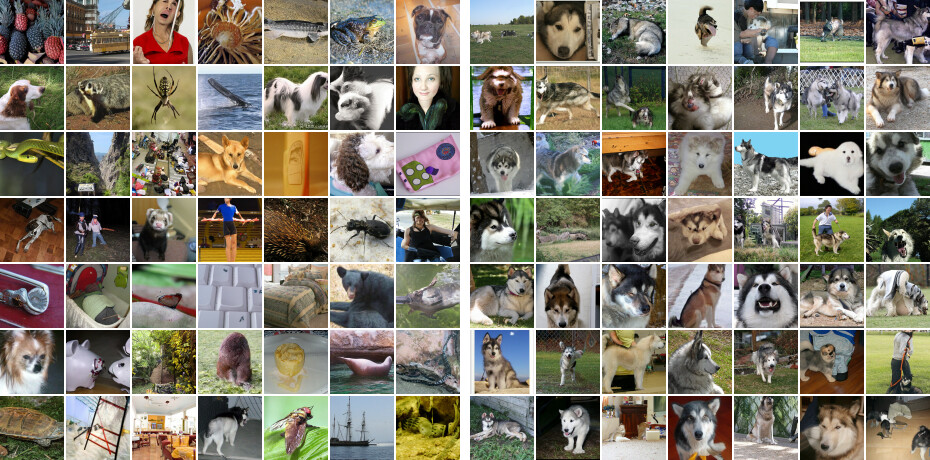
\includegraphics[width=0.9\linewidth]{images/guidance_figure_1_minus0.jpg}
         \caption{
非引导条件抽样:FID=1.80,IS=53.71}
     \end{subfigure}
     \begin{subfigure}[b]{\textwidth}
         \centering
         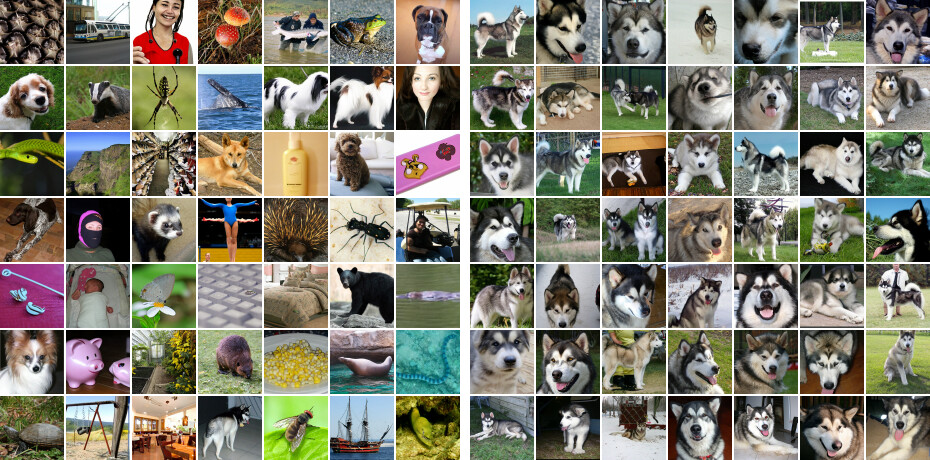
\includegraphics[width=0.9\linewidth]{images/guidance_figure_2_minus1.jpg}
         \caption{
无分类器指南, $w=1.0$ :FID=12.6,IS=170.1}
     \end{subfigure}
     \begin{subfigure}[b]{\textwidth}
         \centering
         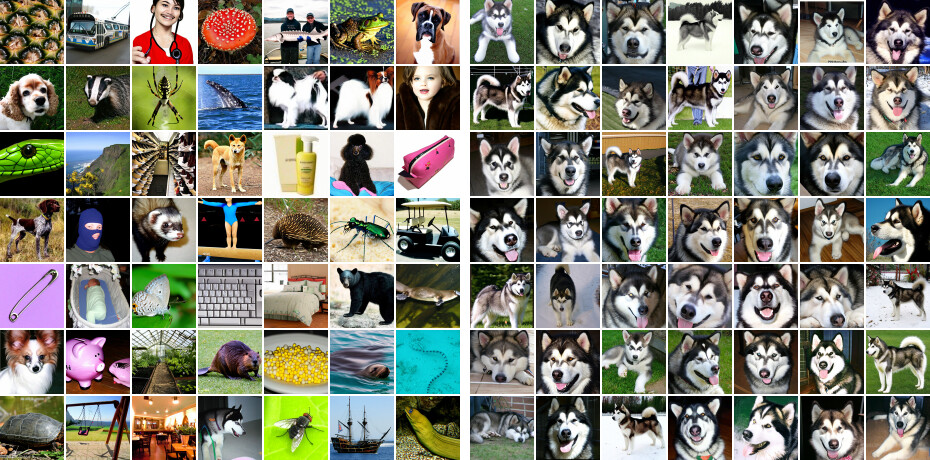
\includegraphics[width=0.9\linewidth]{images/guidance_figure_4_minus3.jpg}
         \caption{
无分类器指南, $w=3.0$ :FID=24.83,IS=250.4}
     \end{subfigure}
        \caption{
ImageNet 64x64上的无分类器指南。左图:随机班。右图:单人班(马拉木舞)。在每个子图中使用相同的随机种子进行抽样。}
        \label{fig:i64_samples}
\end{figure} 


 \begin{figure}[H]\vspace{-1em}
     \centering
     \begin{subfigure}[b]{\textwidth}
         \centering
         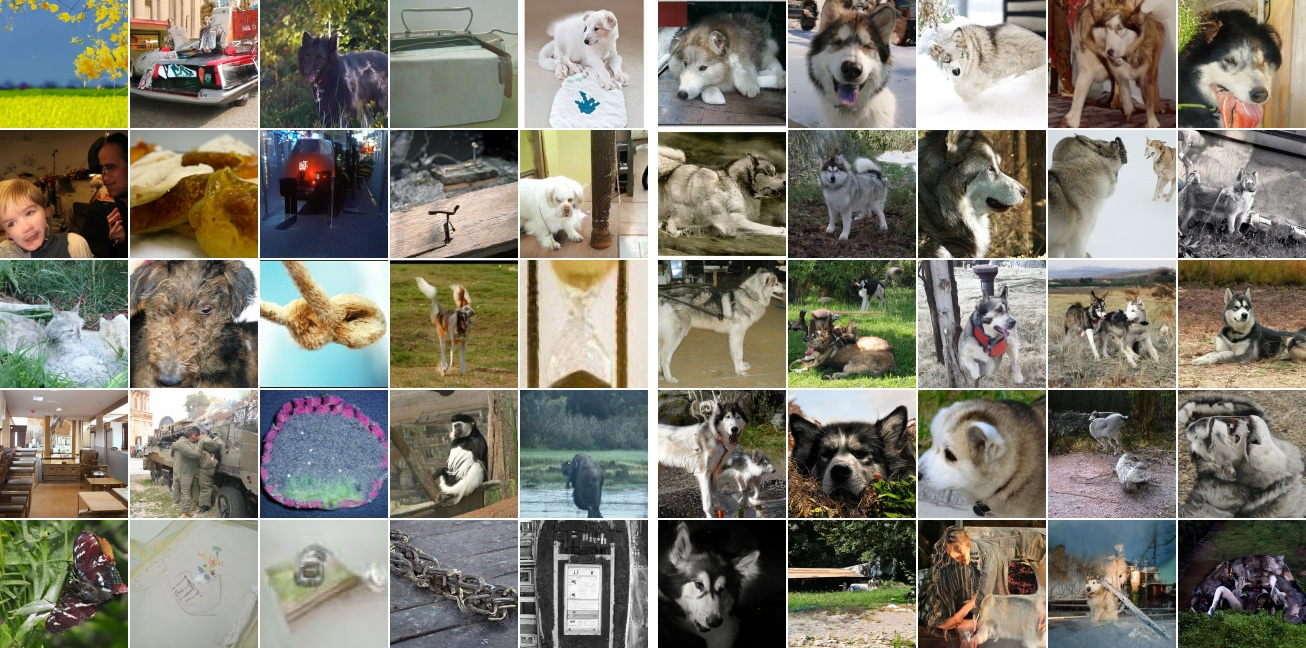
\includegraphics[width=\linewidth]{images/i128_samples_0.jpg}
         \caption{
非引导条件抽样:FID=7.27,IS=82.45}
     \end{subfigure}
     \begin{subfigure}[b]{\textwidth}
         \centering
         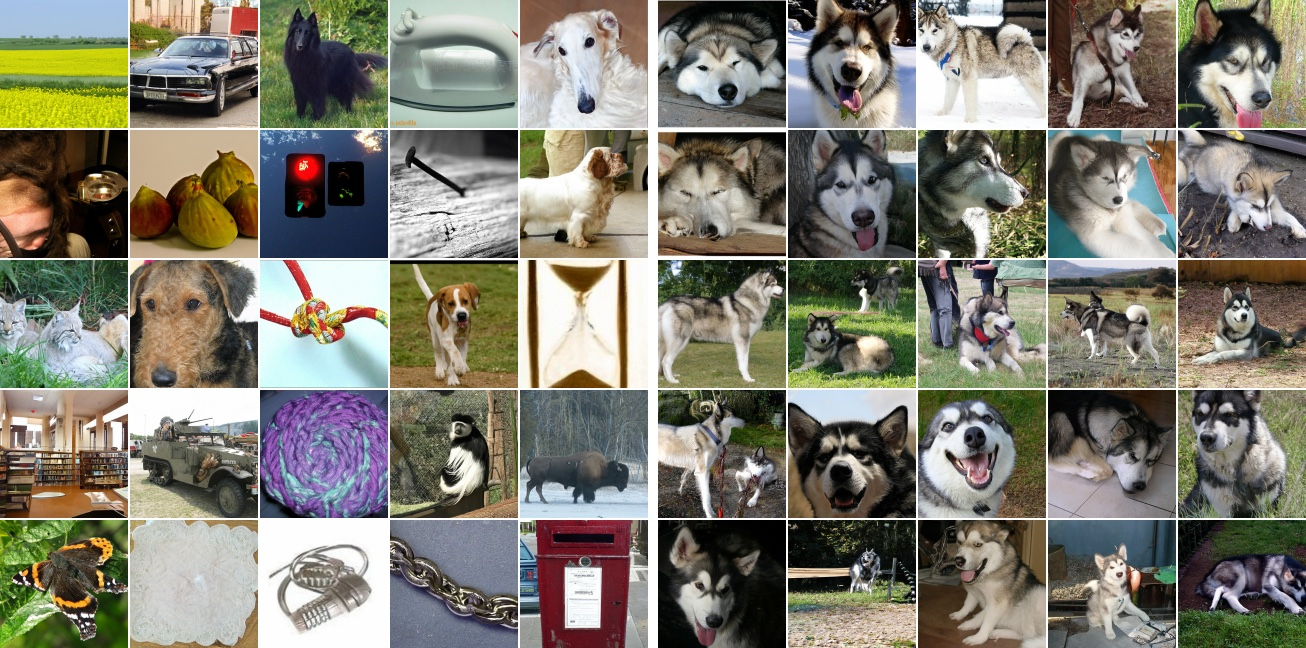
\includegraphics[width=\linewidth]{images/i128_samples_10.jpg}
         \caption{
无分类器指南, $w=1.0$ :FID=7.86,IS=297.98}
     \end{subfigure}
     \begin{subfigure}[b]{\textwidth}
         \centering
         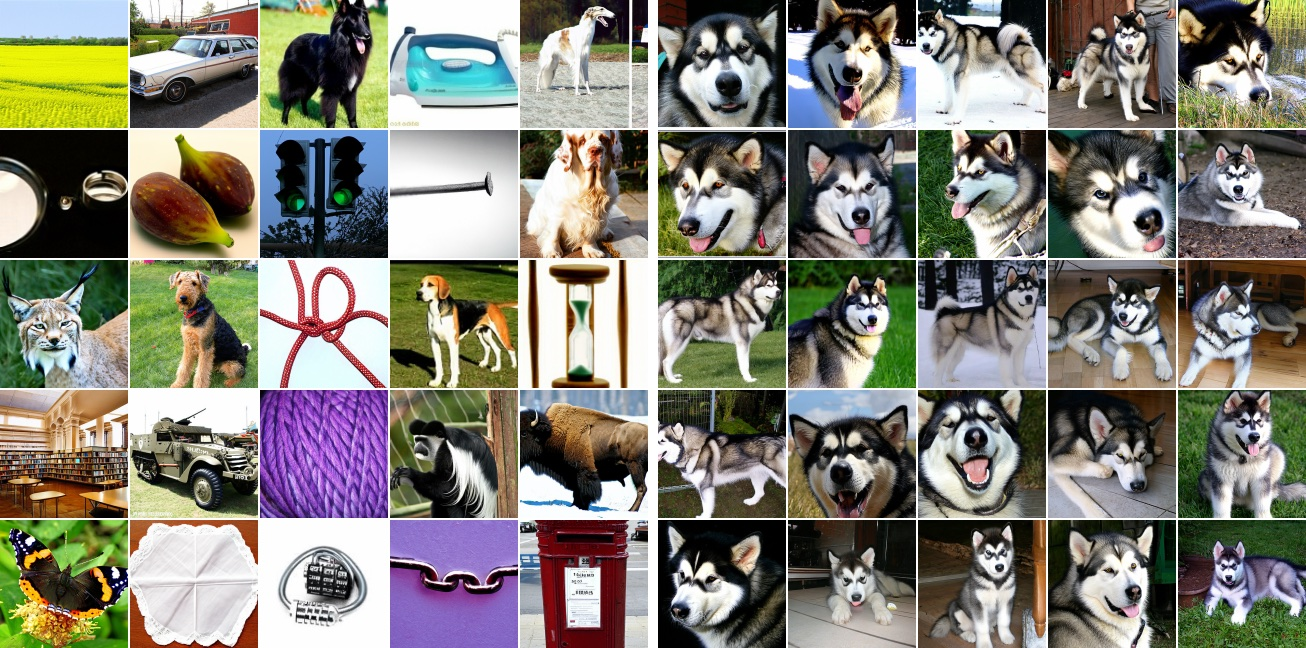
\includegraphics[width=\linewidth]{images/i128_samples_40.jpg}
         \caption{
无分类器指导, $w=4.0$ :FID=21.53,IS=421.03}
     \end{subfigure}
        \caption{
ImageNet 128x128上的无分类器指南。左图:随机班。右图:单人班(马拉木舞)。在每个子图中使用相同的随机种子进行抽样。}
        \label{fig:i128_samples}
\end{figure} 


 \begin{figure}[t] \centering
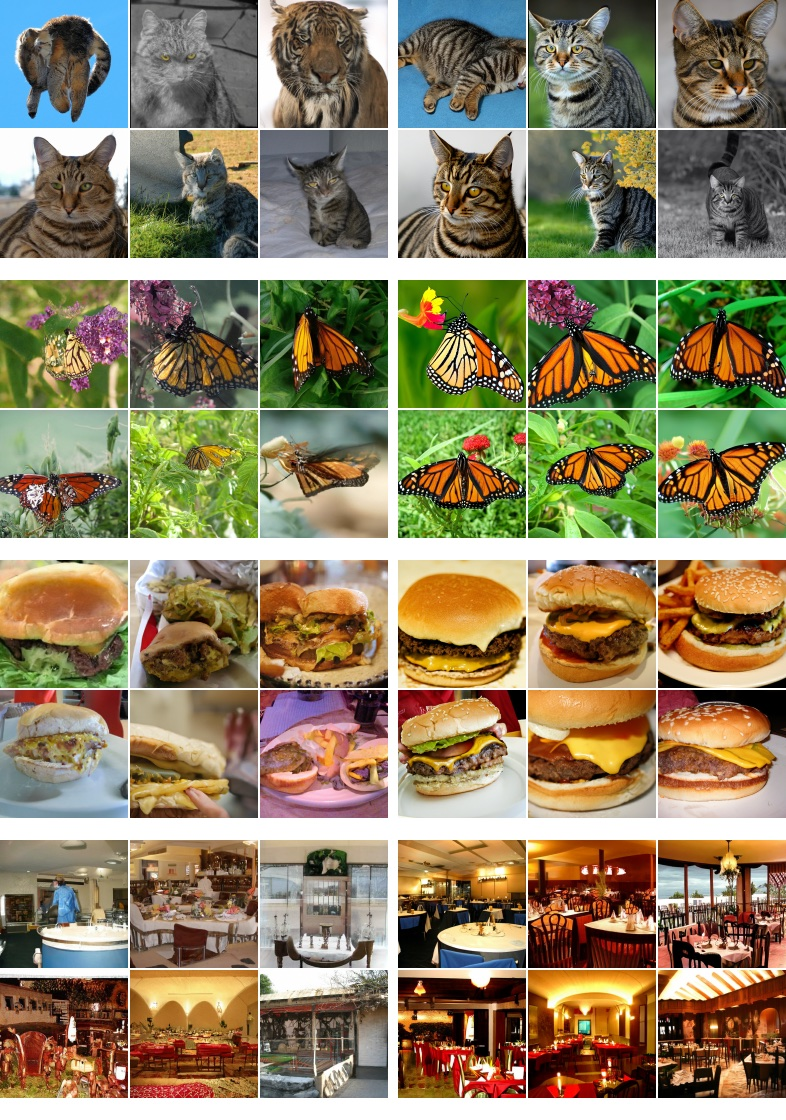
\includegraphics[width=\linewidth]{images/i128_more_samples.jpg}
\caption{
在128x128 ImageNet上提供更多无需分类器的指导示例。左:非引导样本,右:具有 $w=3.0$ 的无分类器引导样本。}
\label{fig:i128_guidance_more}
\end{figure} 



\end{document}

